\Section{Energy Straggling in COSY} \label{sec:COSYStraggling}\par
For energy loss, COSY uses the Bethe-Bloch equation (Eqn. \ref{eqn:bethebloch}) to find the mean energy loss. This can be done in the transfer map paradigm since average energy loss is a deterministic effect. However, this work is concerned with simulating realistic stochastic fluctuations about the average energy loss. For this reason, this work has implemented Landau theory \cite{landau} to describe the straggling distribution. Landau theory is discussed in detail in Section \ref{ssc:ICOOLStragglingLandau}. 

\iffalse
Other straggling models which were investigated were
\begin{itemize}
\item{Functionalization}
\item{Urb\'{a}n model \cite{geant4}}
\item{Vavilov theory \cite{vavilov}}
\item{Edgeworth series \cite{edgeworth}}
\item{Convolution method (compound Poisson method) \cite{kellerer}}
\item{Landau/Gaussian convolution \cite{hancock}}
\item{Blunck-Liesegang theory \cite{blunck}}
\end{itemize}
However, Landau theory proved to be the best fit. It was chosen over the Vavilov distribution in particular due to a complication where the Vavilov tail was abruptly cut off under certain circumstances.
\fi

The average of the Landau distribution is infinity, which is clearly nonphysical. Given the universal Landau parameter (Eqn. \ref{eqn:landauParameter}), 
\begin{align*}
\lambda=\frac{\epsilon-\left<\epsilon\right>}{\xi}-(1-C_{Euler})-\beta ^2 -\ln (\xi/T_{max}),
\end{align*}
fluctuations about the mean energy loss $\left<\epsilon-\left<\epsilon\right>\right>$ will also be divergent given enough samples. The possibility of divergence results in a sensitivity to step size since smaller steps will effectively produce a large sample size. In order to combat this, an artificial cutoff is given to $\lambda$ such that the average Landau $\epsilon$ is equal to the average Bethe-Bloch energy loss $\left<\epsilon\right>$. That is, it is required that
\begin{align*}
\left<\lambda\right>&=\left<\frac{\epsilon-\left<\epsilon\right>}{\xi}\right>-(1-C_{Euler})-\beta^2-\ln(\xi/T_{max})\\
&=-(1-C_{Euler})-\beta^2-\ln(\xi/T_{max}).
\end{align*}
If this cutoff is $\lambda_{max}$, then $\left<\lambda\right>$ can be calculated by the definition of an average over the range $[0,\lambda_{max}]$:
\begin{align*}
\left<\lambda\right>=\frac{\int_0 ^{\lambda_{max}} \lambda * f(\lambda) d\lambda}{\int_0 ^{\lambda_{max}}f(\lambda) d\lambda}.
\end{align*}
The task then is to numerically find $\lambda_{max}$ such that it satisfies
\begin{align*}
\frac{\int_0 ^{\lambda_{max}} \lambda * f(\lambda) d\lambda}{\int_0 ^{\lambda_{max}}f(\lambda) d\lambda}=-(1-C_{Euler})-\beta^2-\ln(\xi/T_{max}).
\end{align*}
GEANT version 3.21 \cite{geant3.21} suggests the following form for $\lambda_{max}$:
\begin{equation} \label{eqn:landauCutoffsGeant3}
\lambda_{max}=0.60715+1.1934\left<\lambda\right>+(0.67794+0.052382\left<\lambda\right>)\exp[0.94753+0.74442\left<\lambda\right>)]
\end{equation}
(note that GEANT4 does not have a section on the Landau cutoff since the Urb\'{a}n model is used instead). However, a plot of required cutoffs ($\lambda_{max}$) vs. desired means ($\left<\lambda\right>$) was produced independently in this work with muon ionization cooling parameters in mind. The form suggested by GEANT3 (see, e.g., Eqn. \ref{eqn:landauCutoffsGeant3}) was used to fit the plot in Figure \ref{fig:landau_cutoffs}. The determined form of the function is
\begin{equation}\label{eqn:landauCutoffs}
\lambda_{max}=0.517891+1.17765\left<\lambda\right>+(0.476074+0.00880733\left<\lambda\right>)\exp[1.15467+0.984008\left<\lambda\right>].
\end{equation}

\begin{figure}
  \centering
    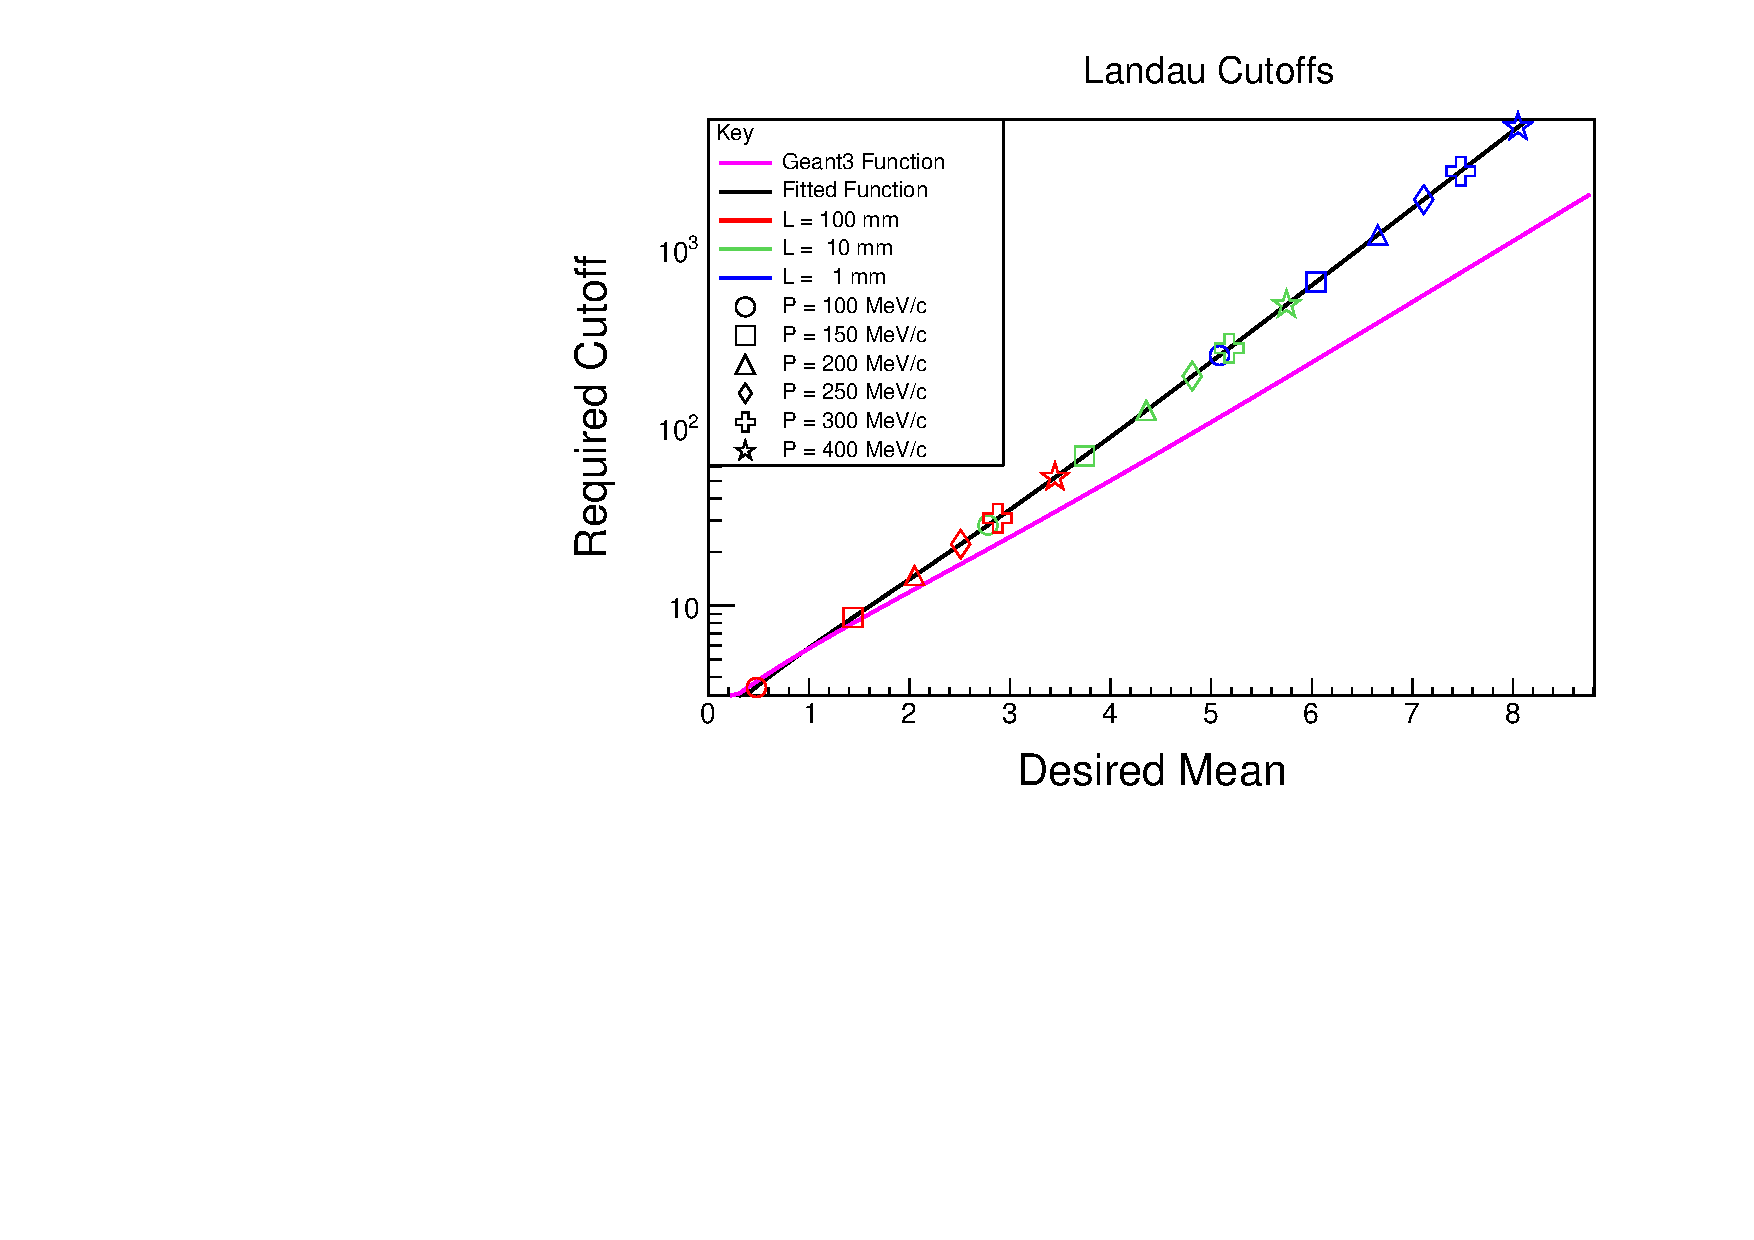
\includegraphics[width=\textwidth]{Figures/landau_cutoffs} 
  \caption[$\lambda_{max}$ vs. $\left<\lambda\right>$ over a variety of liquid hydrogen absorber lengths and initial beam momenta.]{$\lambda_{max}$ vs. $\left<\lambda\right>$ over a variety of liquid hydrogen absorber lengths and initial beam momenta. The pink line is the form given by GEANT3 (see Eqn. \ref{eqn:landauCutoffsGeant3}) and the black line is the fitted curve (see Eqn. \ref{eqn:landauCutoffs}).}
  \label{fig:landau_cutoffs}
\end{figure}

Based on Eqn. \ref{eqn:landauParameter}, it is possible to find $\epsilon_{max}$:
\begin{align*}
\epsilon_{max}=\xi[\lambda_{max}+(1-C_{Euler})+\beta^2+\ln(\xi/T_{max})]+\left<\epsilon\right>.
\end{align*}
Therefore, during the energy loss sampling, if any energy loss $\epsilon$ is selected which is greater than $\epsilon_{max}$ it is thrown out and the sampling is performed again. However, if the result has been thrown out 100 times, the particle is assumed to have lost too much energy and is considered lost.

%
%-------------------------------------------------------------------------------
%
\Section{Multiple Scattering in COSY Infinity} \label{sec:COSYScattering}\par
Similar to ICOOL's fifth method of scattering, the Rutherford model (see Sec. \ref{sec:ICOOLScattering}), COSY utilizes a piecewise distribution function which is Gaussian  at small angles (as Goudsmit and Saunderson suggested \cite{gs}) and Rutherford-like at large angles. This Ruthorford-like tail is derived at length in Appendix \ref{apx:cosy_cross_section}, with a review of the relevant particle physics symbols and methods in Appendix \ref{apx:particlePhysicsReview}. The result is the (differential) Mott scattering cross section:
\begin{equation}\label{eqn:MottCrossSection}
\frac{d\sigma}{d\Omega} \propto \frac{1+\frac{(\beta\gamma)^2}{2} (1+\cos\theta)  }{(1-\cos\theta)^2},
\end{equation}
where $d\sigma/d\Omega$ is the differential scattering cross section, $\beta$ is the relativistic velocity, $\gamma=1/\sqrt{1-\beta^2}$, and $\theta$ is the scattering angle. Observe that for the non-relativistic limit $\beta\rightarrow 0$ the cross section does indeed approach a Rutherford distribution (Eqn.\ref{eqn:rutherford}). The practical implementation of this cross section into the probability distribution function is then discussed in Sec. \ref{ssc:COSYScatteringImplementation}.

\Subsection{Implementation}\label{ssc:COSYScatteringImplementation} Now that the forms of the Gaussian and Rutherford-like scattering cross sections have been obtained, implementation of these cross sections will be discussed. In COSY, when a particle passes through matter, the change in angle of this particle is selected from a probability distribution. For $u=\cos\theta$, this distribution should be Gaussian-like at small angles \cite{gs} and follow the Mott cross section at large angles. Based on a Gaussian-like cross section for small angles and the cross section in Eqn. \ref{eqn:MottCrossSection}, the distribution has been chosen as
\begin{align}\label{eqn:cosyg}
g(u)=	\begin{cases}
	e^{-a(1-u)} & \quad u_0 ,\leq u \\
	\zeta\frac{1+\frac{1}{2}(\beta\gamma)^2(1+u-b_c)}{(1-u+b_c)^2} & \quad u\leq u_0
	\end{cases},
\end{align}
where $u_0$ is the cutoff between the Gaussian-like distribution and the Mott distribution, $\zeta$ is the amplitude of the Mott distribution, and $b_c$ is the relative $u$ shift of the Mott distribution. The parameter $a$ is an empirical parameter, based off Highland theory \cite{highland}, and can be found in Eqn. \ref{eqn:geanta}. Eqn. \ref{eqn:geanta} is reproduced here for convenience:
\begin{align*}
a=\frac{0.5}{1-\cos\theta_0}.
\end{align*}
where $\theta_0$ has the form \cite{highland} 
\begin{align*}
\theta_0 = \frac{E_s}{p\beta} \sqrt{\frac{L}{X_0}}.
\end{align*}
However, this definition has been extended in this work to include empirical corrections based on GEANT4's \cite{geant4} treatment of $\theta_0$ (see Eqn. \ref{g4bltheta0}):
\begin{equation}\label{eqn:cosytheta0}
\theta_0 = \frac{13.6 \text{ eV}}{\beta p} \sqrt{\frac{L}{X_0} \Big[ 1+h_1 \ln \frac{L}{X_0} + h_2 \Big(\ln \frac{L}{X_0}\Big)^2 \Big] }.
\end{equation}
The Highland correction terms have been chosen novelly in this work as $h_1=0.103$ and $h_2=0.0038$. 
%This was done by fitting the curve given by Eqn. \ref{eqn:cosyg} to match the MuScat results \cite{muscat}.

$u_0$ is the point at which the Gaussian term meets the Mott tail. This has been chosen empirically as
\begin{equation}\label{eqn:cosyu0}
u_0=1-\frac{4.5}{a}.
\end{equation}
This parameter was fitted alongside the Highland correction terms to match the experimental results in \cite{muscat}.

$\zeta$ and $b_c$ are the angular scattering distribution's amplitude and offset for the tail. These are found by demanding continuity and smoothness at $u_0$:
\begin{align*}
e^{-a(1-u_0)}&=\zeta\frac{1+\frac{1}{2}(\beta\gamma)^2(1+u_0-b_c)}{(1-u_0+b_c)^2},\\
ae^{-a(1-u_0)}&=\zeta\frac{1+\frac{1}{2}(\beta\gamma)^2(1+u_0-b_c)}{(1-u_0+b_c)^2} \Big(\frac{2}{1-u_0+b_c}+\frac{(\beta\gamma)^2}{2+(\beta\gamma)^2(1+u_0-b_c)}\Big).
\end{align*}
Then
\begin{align*}
a=\frac{2}{1-u_0+b_c}+\frac{(\beta\gamma)^2}{2+(\beta\gamma)^2(1+u_0-b_c)}.
\end{align*}
Solving this for $(u_0-b_c)$ yields a quadratic with the solution
\begin{align} \label{eqn:cosybc}
b_c=u_0+\frac{A_2 + \sqrt{A_2 ^2 - 4A_1 A_3}}{2A_1},
\end{align}
with
\begin{align*}
A_1=&-a(\beta\gamma)^2,\\
A_2=&-(\beta\gamma)^2-2a,\\
A_3=&(\beta\gamma)^2(a-3)+2a-4.
\end{align*}
The constraint for continuity of $g(u_0)$ can now be solved to find $\zeta$:
\begin{equation}\label{eqn:cosyzeta}
\zeta=\frac{e^{-a(1-u_0)}(1-u_0+b_c)^2}{1+\frac{1}{2}(\beta\gamma)^2(1+u_0-b)}.
\end{equation}

Now that the distribution function has a concrete form, it is implemented by inverting the cumulative distribution function (CDF).  Let $G(u)$ be the integral of $g(u)$. Then the variable $G$ will be uniformly sampled over the region $[0,G_{max}]$. If $G\geq G(u_0) \equiv G_0$ then the Gaussian part of the distribution is used to generate $u$ (i.e. $G(u\geq u_0)$). Otherwise, the tail of the distribution is used. Figure \ref{fig:scatdist_example} shows $G(u)$ for $L=100$ mm, $p=200$ MeV/$c$, and a radiation length of $X_0 = 8.66$ m (to simulate a liquid hydrogen target).

\begin{figure}
  \centering
    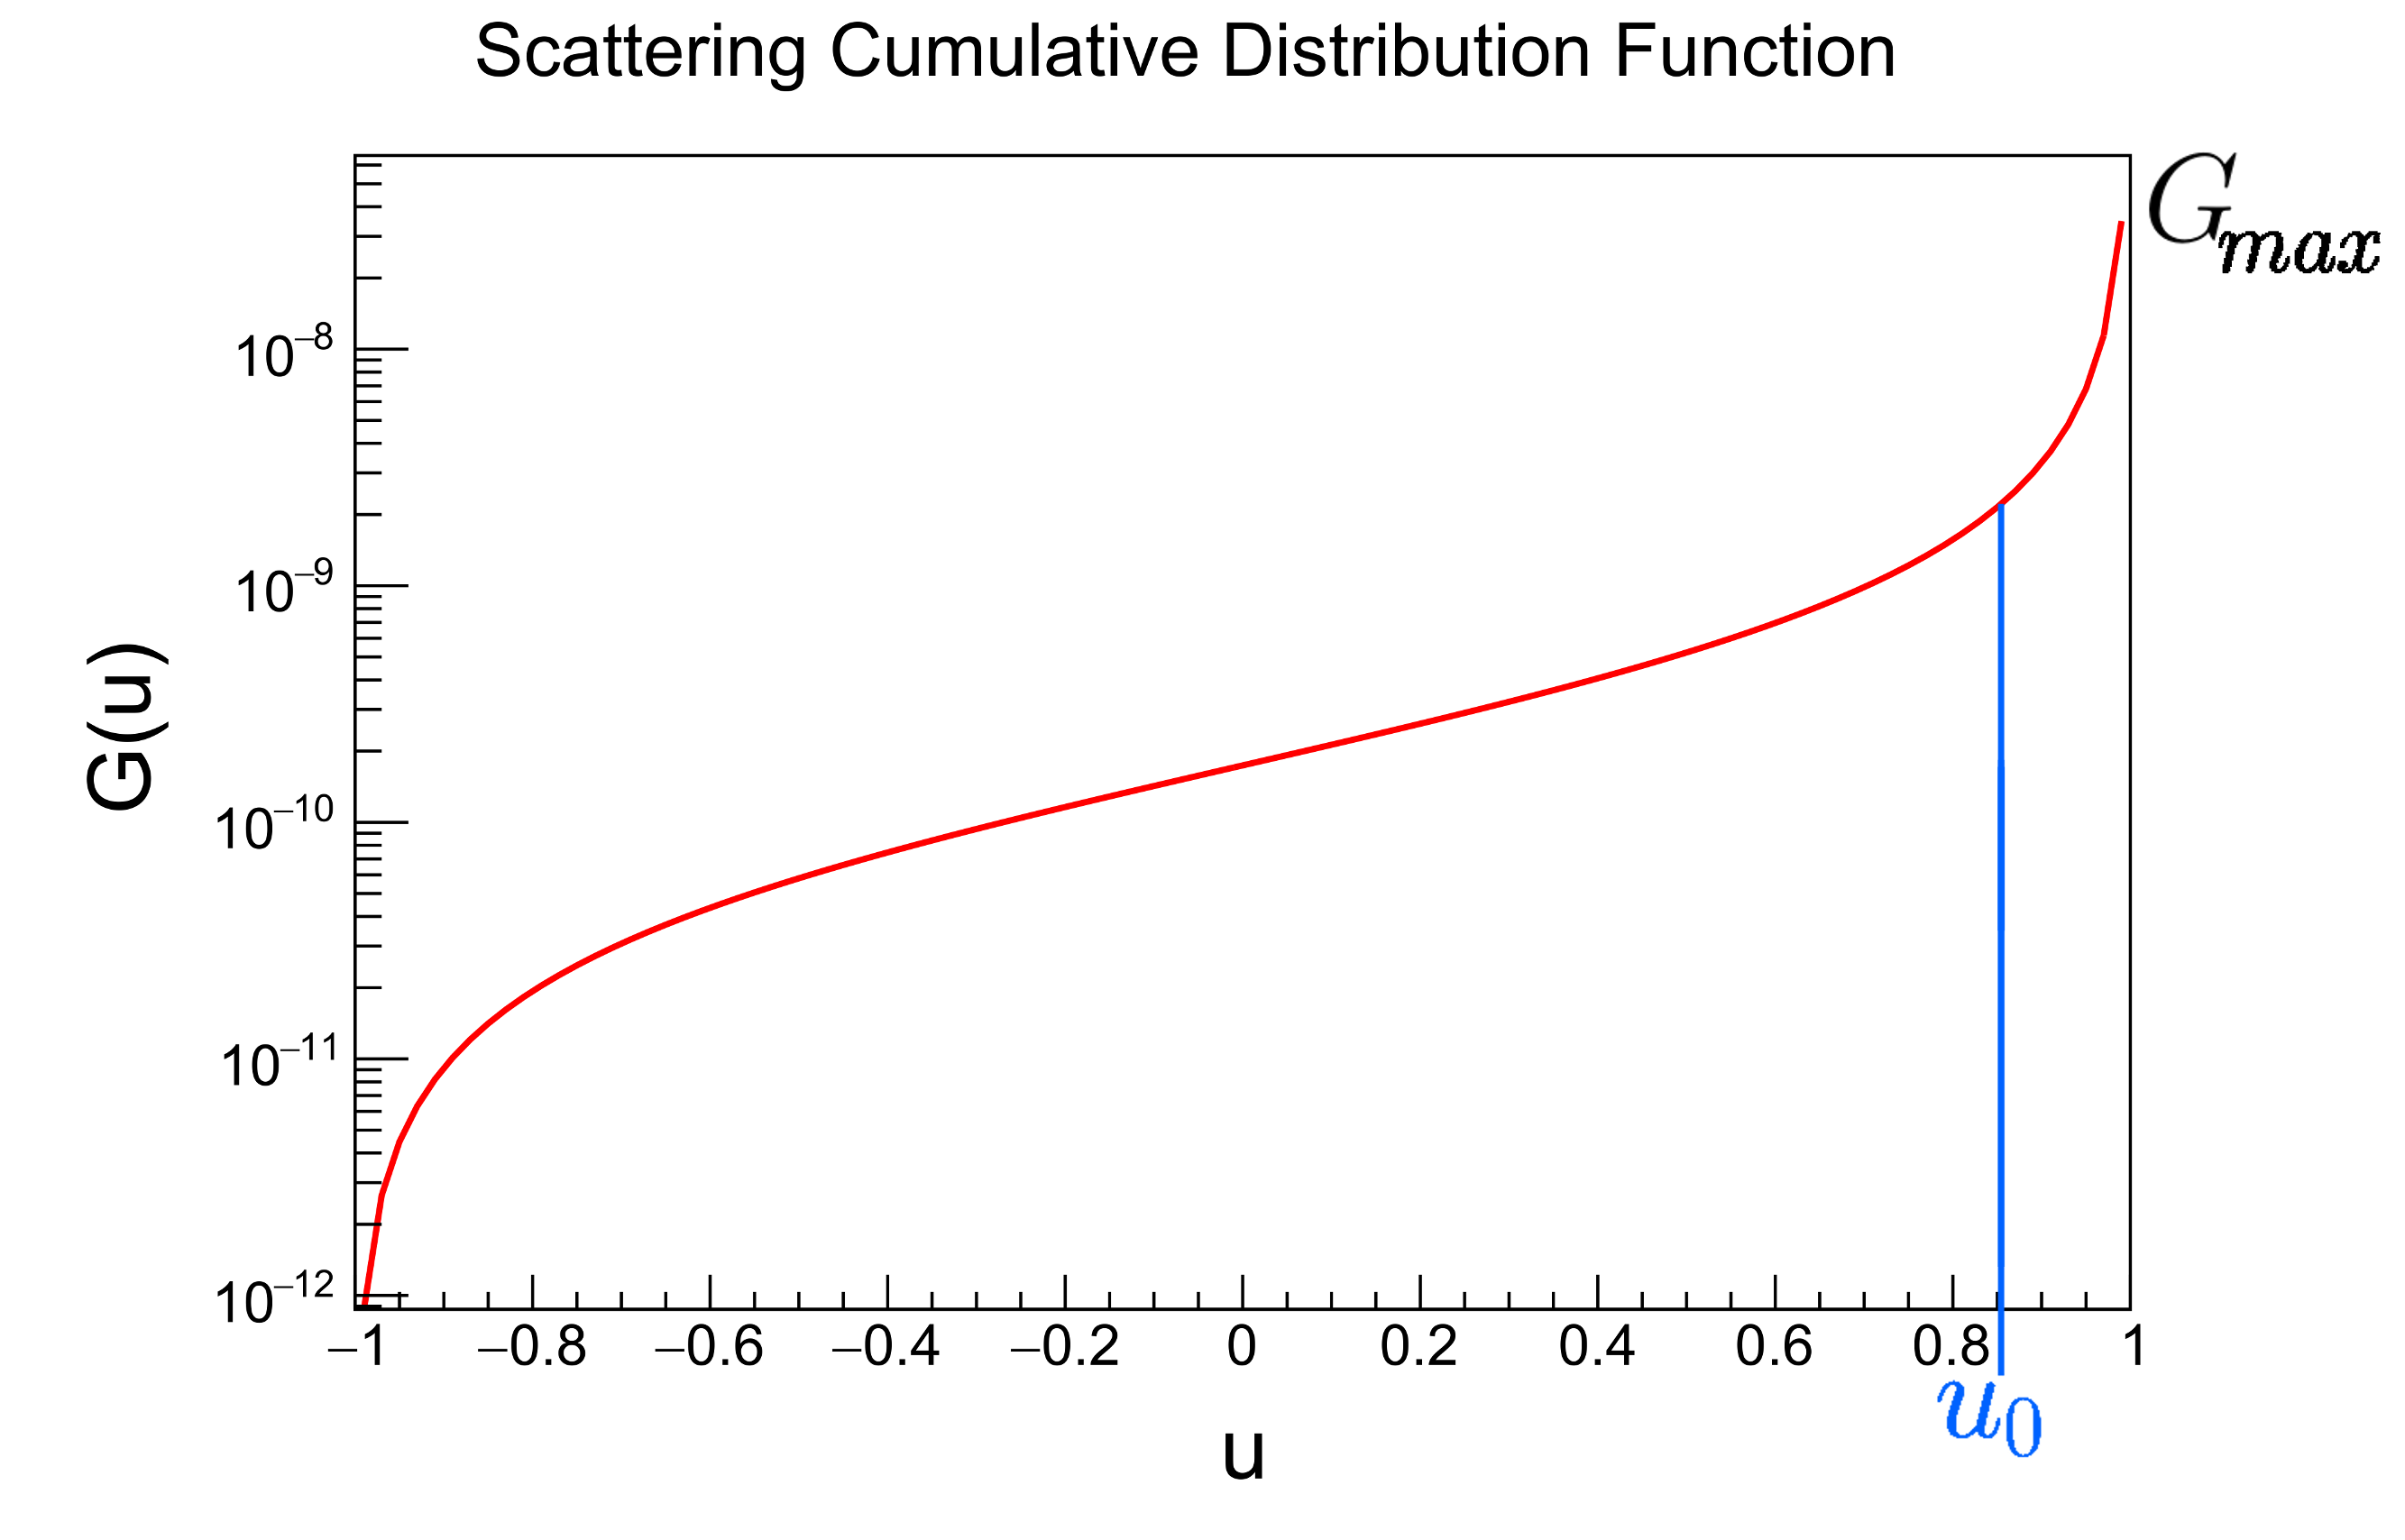
\includegraphics[width=\textwidth]{Figures/scatdist_example} 
  \caption[Example of the COSY cumulative angular distribution function.]{Example of the cumulative angular distribution function for muons with momenta of 200 MeV/$c$ through 100 mm of liquid hydrogen. Note that the $y$ axis is log scaled due to the very sharp peak. Furthermore, note that $u_0$ is greatly exaggerated, since its actual value for these parameters is 0.99987.}
  \label{fig:scatdist_example}
\end{figure}

However, since this is a piecewise function, the CDF will be inverted in pieces. The tail of the CDF will be found first:
\begin{align*}
G(u\leq u_0)=\int _{-1} ^u \zeta \frac{1+\frac{1}{2}(\beta\gamma)^2 (1+u'-b_c)}{(1-u'+b_c)^2} du'.
\end{align*}
This integral may be solved by substituting $v=1-u'+b_c$ and simply splitting the numerator into separate parts:
\begin{align}
\nonumber
G(u\leq u_0)=&-\zeta(1+\frac{1}{2}(\beta\gamma)^2(1-b_c))\int_{2+b_c} ^{1-u+b_c} v^{-2} dv - \\
\nonumber
& \quad \zeta \frac{(\beta\gamma)^2}{2}\int_{2+b_c} ^{1-u+b_c} (v^{-2} - v^{-1} + b_c v^{-2}) dv\\
G(u\leq u_0)=&\zeta(1+(\beta\gamma)^2)\left(\frac{1}{1-u+b_c} - \frac{1}{2+b_c}\right)+\zeta \frac{(\beta\gamma)^2}{2} \ln\Big(\frac{1-u+b_c}{2+b_c}\Big) \label{eqn:cosyGTail}
\end{align}

The goal is to solve Eqn. \ref{eqn:cosyGTail} for $u(G)$. However, using direct inversion is extremely difficult and involves special functions. Therefore, it is more prudent to generate  $u$ via bisection method (see Figure \ref{fig:scatdist_algorithm}). In this method, the true $G$ is sampled uniformly on the range $[0,G_{max}]$, where $G_{max} \equiv G(1)$. Explicitly, $G_{max}$ is
\begin{align*}
G_{max}\equiv G(1) &=\int_{-1} ^{u_0} \zeta\frac{1+\frac{1}{2}(\beta\gamma)^2(1+u-b_c)}{(1-u+b_c)^2}du+\int_{u_0} ^1 e^{-a(1-u)} du,\\
&= G_0+\frac{1}{a}-\frac{e^{-a(1-u_0)}}{a}.
\end{align*}
If $G < G_0$, then the tail is sampled. A trial $u$ called $\bar{u}$ (as in `average') is selected from some range which is known to contain the actual $u$. The range is described as $[u_{min},u_{max}]$, and $\bar{u}=(u_{min}+u_{max})/2$. 

Initially, the range is chosen as $u_{min}=-1$ and $u_{max}=u_0$ (since that is the largest range on which $G(u \leq u_0)$ is valid and hence $u$ is guaranteed to be in this range). $\bar{G} \equiv G(\bar{u})$ is found using Eqn. \ref{eqn:cosyGTail}, and then the routine is subject to the following conditions:
\begin{align*}
&\text{If } \bar{G}\in [G-\delta G,G+\delta G] &\quad &\text{then } u=\bar{u}\text{, return value.}\\
&\text{If } \bar{G} < G-\delta G &\quad &\text{then } u_{min}=\bar{u} \text{, rerun with new }u_{min}.\\
&\text{If } \bar{G} > G+\delta G &\quad &\text{then } u_{max}=\bar{u} \text{, rerun with new }u_{max}.
\end{align*}
$\delta G$ is a precision, and has been chosen for this work as $\delta G = 10^{-8}$. However, it is conceded that in the future $\delta G$ should be a percentage of $G_{max}$ rather than an absolute number.

\begin{figure}
  \centering
    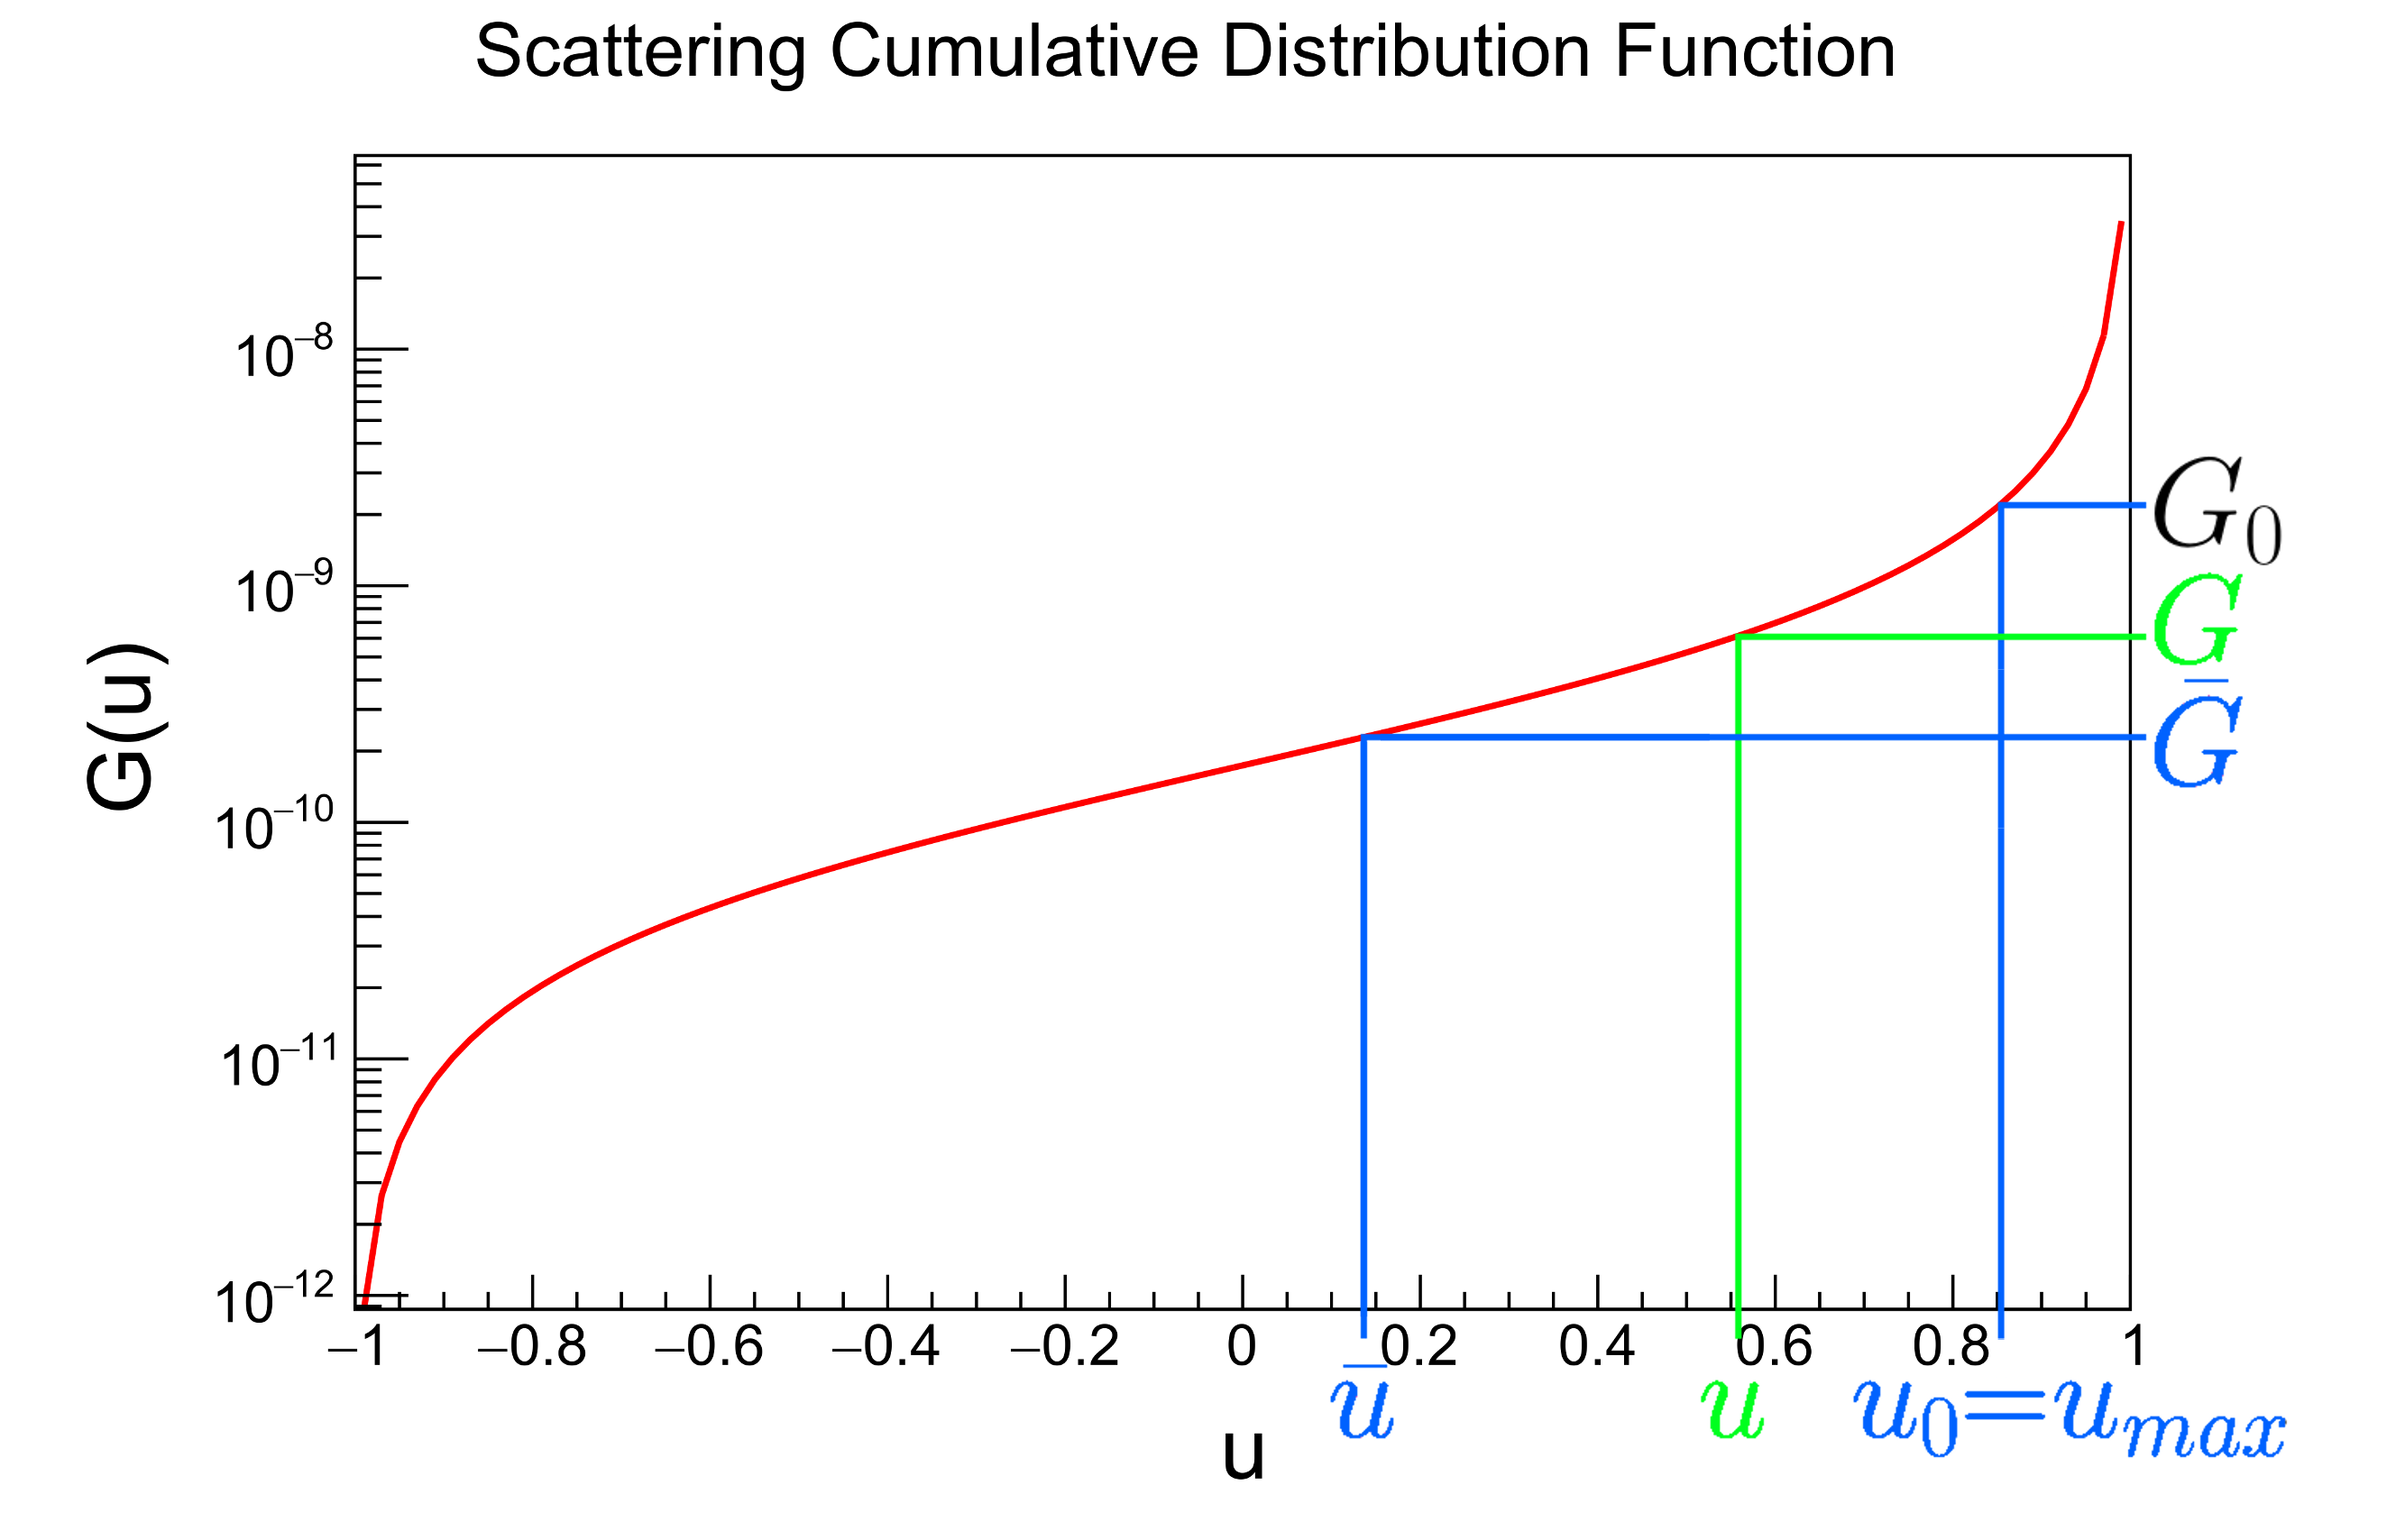
\includegraphics[width=\textwidth]{Figures/scatdist_algorithm} 
  \caption[Example of the first iteration of the COSY CDF algorithm.]{Example of the first iteration of the algorithm to obtain the true $u$ (in green). The true $G$ is chosen uniformly from $G\in[0,G_{max}]$. If $G < G_0$, then the tail is sampled via bisection method. In this case, since $\bar{G} < G$, $\bar{u}$ is the new $u_{min}$ and $\bar{u}$ is calculated again.}
  \label{fig:scatdist_algorithm}
\end{figure}

For the peak, $u_0 \leq u$ and so the CDF becomes
\begin{align*}
G(u_0 \leq u)&=\int_{-1} ^{u_0} g(u) du + \int_{u_0} ^u e^{-a(1-u)} du.
\end{align*}
The first term is simply $G_0$, the cumulative distribution function at $u_0$. The second term is easily integratable and yields
\begin{equation}\label{eqn:cosyGPeak}
G(u_0 \leq u)=G_0 + \frac{e^{-a(1-u)}-e^{-a(1-u_0)}}{a}.
\end{equation}
The inversion of this function is quite straightforward, and is
\begin{equation} \label{eqn:cosyGPeakInverted}
u(G_0 \leq G)=1+\frac{1}{a} \ln \left[a(G-G_0)+e^{-a(1-u_0)}\right].
\end{equation}
Therefore, if $G \in [0,G_{max}]$ is greater than or equal to $G_0$, then it is simply inserted into Eqn. \ref{eqn:cosyGPeakInverted} and the true $u$ is obtained.

It is a subtle yet important point to note that the Mott cross section (Eqn. \ref{eqn:MottCrossSection}), upon which the probability distribution function $g(u)$ in Eqn. \ref{eqn:cosyg} is based, assumes an on-axis straight line trajectory (that is, $x=y=p_x = p_y =0$). The treatment of this subtlety will be discussed here.

The implemented routine for this work which uses the scattering distribution $g(u)$ is called SCATDIST. This routine takes two arguments: $\theta_0$ (Eqn. \ref{eqn:cosytheta0}) and $p$, the total momentum. $\theta_0$ includes not only the material parameters ($L, X_0$) but also energy terms ($1/\beta p$), and $p$ is the momentum \textit{after} the straggling routine has been called. SCATDIST returns not the scattered angle, but the new z-momentum $p_z=pu=p\cos\theta$. 

This new z-momentum is in the rotated frame, i.e. the frame at which $p_x=p_y=0$ (see Figure \ref{fig:cosyRotatedFrame}), and so is called $p_{z,R}$. The transverse momentum in the rotated frame, $p_{T,R}$, can be found via $p_{T,R}=\sqrt{p^2-p_{z,R}^2}$, but this is the total transverse momentum ($\theta_o + \theta_s$), which includes the original momentum ($\theta_o$), not simply the transverse momentum which was gained via scattering ($\theta_s$). Rotation back into the lab frame is given by
\begin{align*}
\begin{pmatrix}
P_{z} \\ P_T
\end{pmatrix}
=
\begin{pmatrix}
\cos\theta_o & -\sin\theta_o\\
\sin\theta_o & \cos\theta_o
\end{pmatrix}
\begin{pmatrix}
P_{z,R} \\ P_{T,R}
\end{pmatrix}.
\end{align*}

\begin{figure}
  \centering
    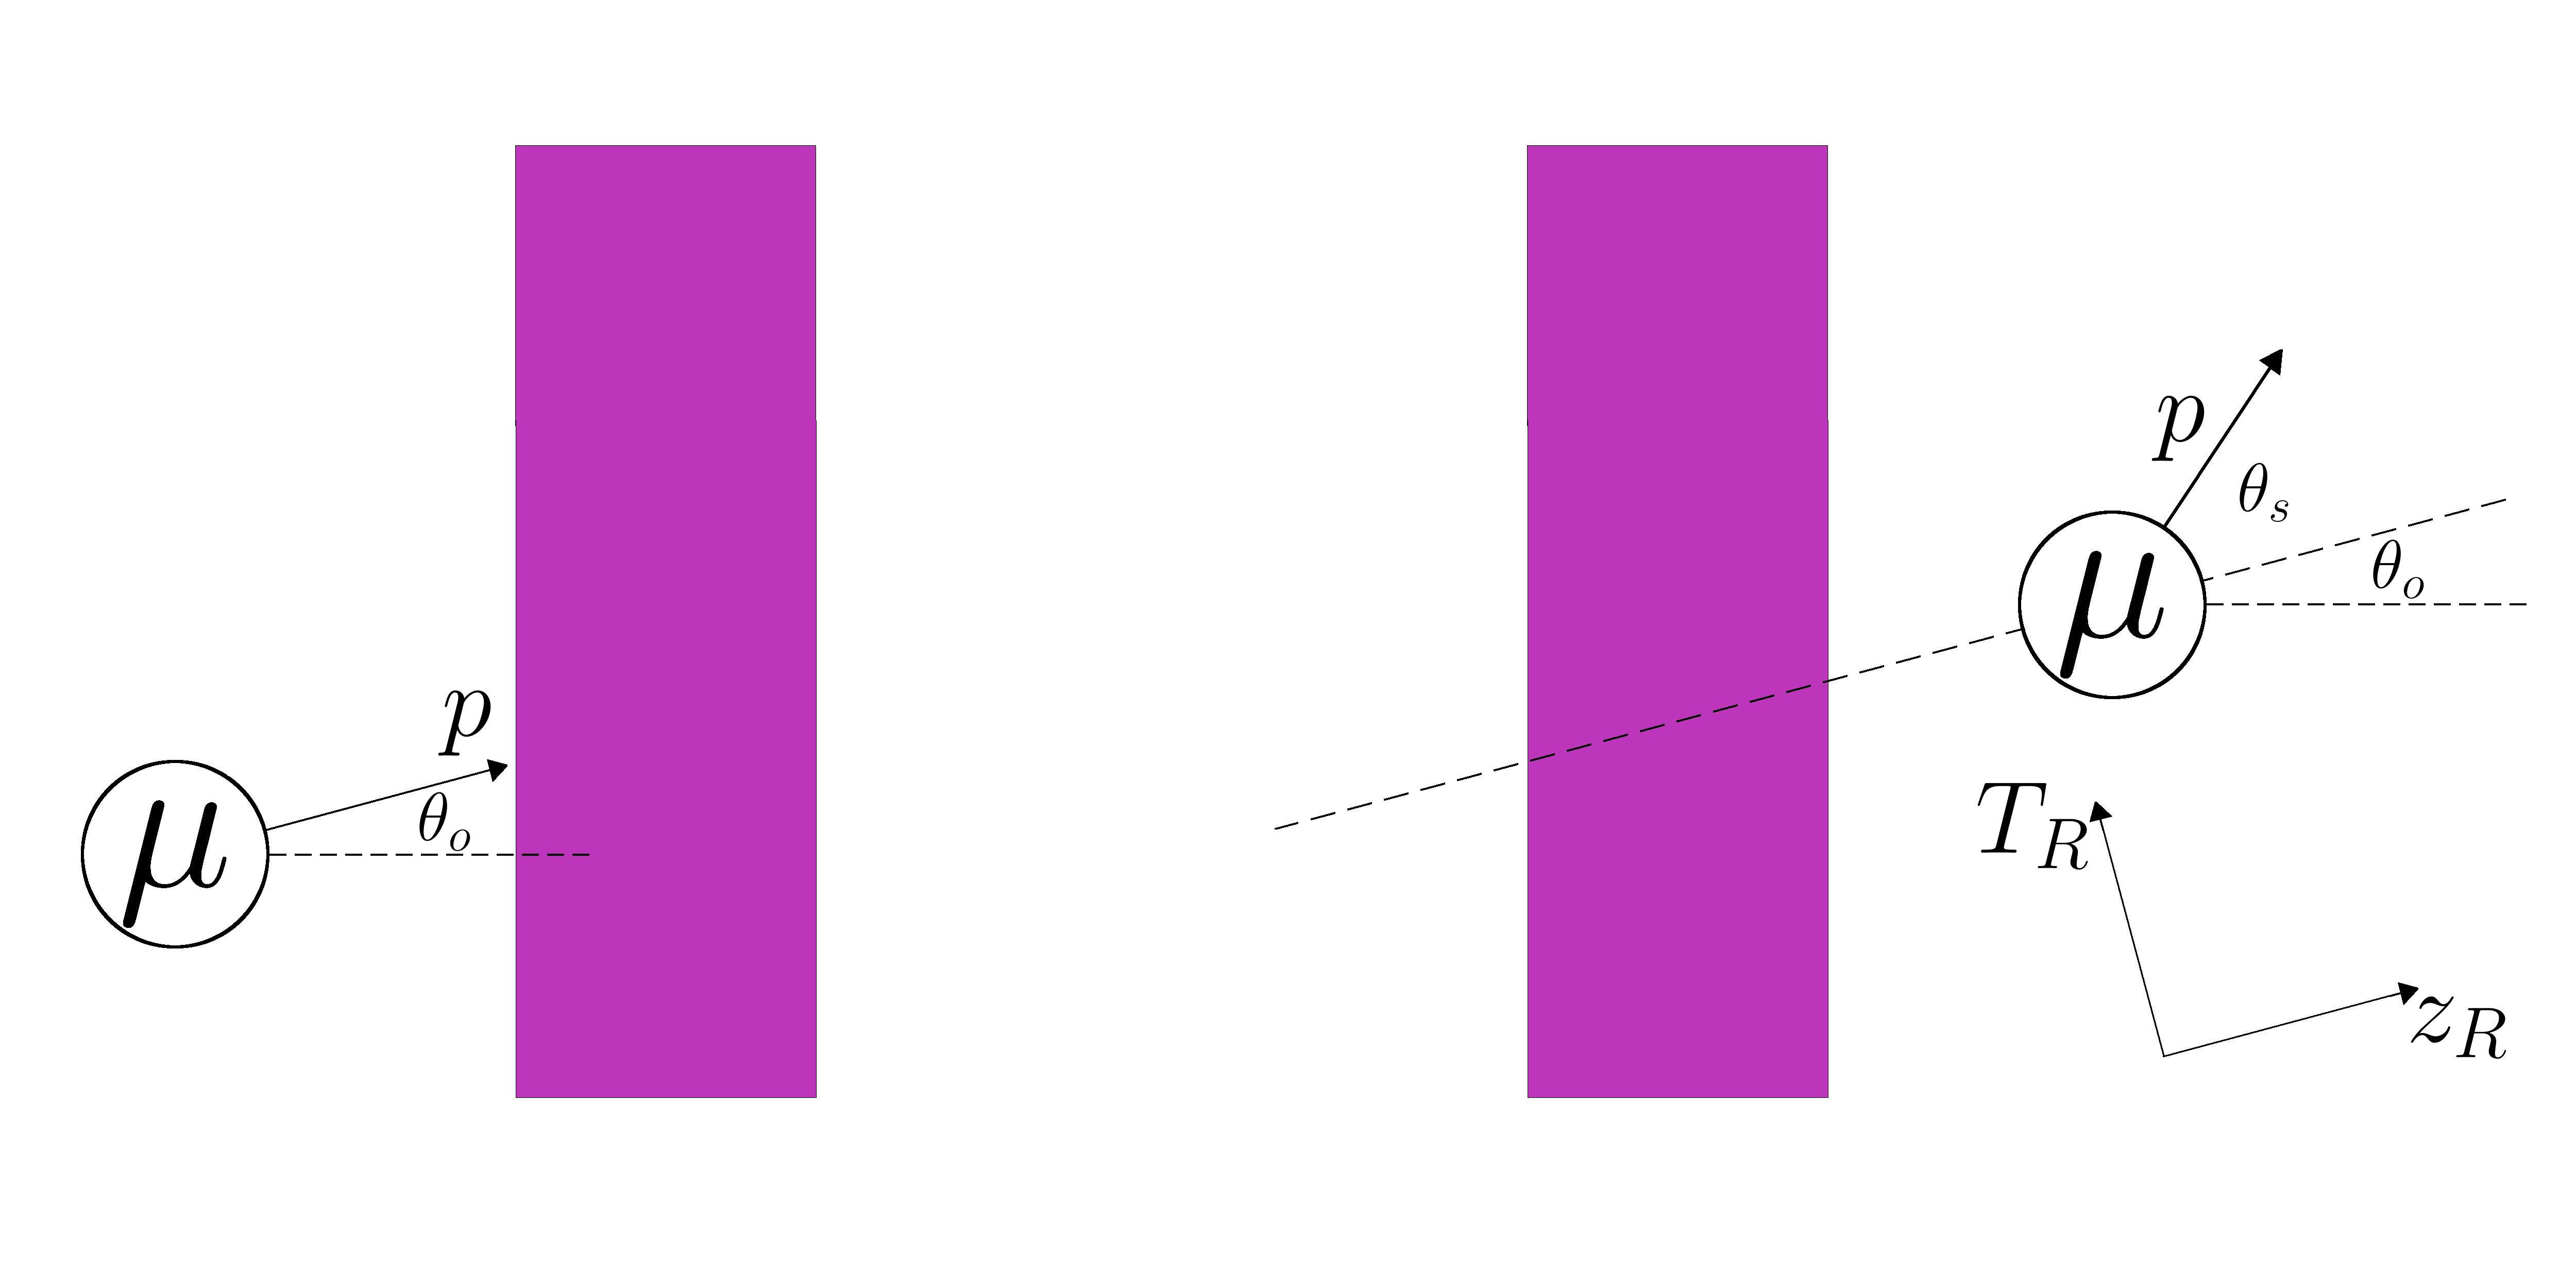
\includegraphics[width=\textwidth]{Figures/cosyRotatedFrame} 
  \caption[Example of a muon entering an absorber with some nonzero initial angle.]{Example of a muon entering an absorber (purple) with some nonzero initial angle $\theta_o$. The muon then scatters an angle $\theta_s$ with respect to its inital momentum $\vec{p}$. The scattering distribution $g(u)$ assumes a straight, on-axis particle ($x=y=p_x=p_y=0$), and so is in the rotated frame, represented by $T_R, z_R$.}
  \label{fig:cosyRotatedFrame}
\end{figure}

Note that at this point one must not uniformly distribute $P_T$ into $p_x$ and $p_y$. This is because, for example, if $p_x$ was positive before scattering it should have a strong probability of being positive after scattering. If one were to distribute $P_T$ uniformly then $p_x$ would have a 50/50 chance of being negative. While the histogram of $p_x$ may not be affected, the transverse phase space would certainly not be correct. For this reason, only the transverse momentum gained via scattering should be uniformly distributed into $p_x$ and $p_y$.

Let the original momenta (after straggling but before scattering) be denoted with $o$ in the same fashion that $\theta_o$ is the angle before scattering. Then the amount of transverse momentum which was gained via scattering is $P_T-P_{T,o}$. This new amount of transverse momentum must be added to the original $p_{x,o}$ and $p_{y,o}$ uniformly. Consequently, let $\phi$ be an angle chosen from $[0,2\pi]$. Then the final $p_x$ and $p_y$ are
\begin{align*}
p_x&=p_{x,o}+(P_T-P_{T,o})\cos\phi\\
p_y&=p_{y,o}+(P_T-P_{T,o})\sin\phi.
\end{align*}

In summation, the angular distribution used by COSY Infinity is based on a piecewise function which is Gaussian for small angles \cite{gs} and has a Mott tail for large angles. This distribution is represented by $g(u)$ in Eqn. \ref{eqn:cosyg}, where $u\equiv \cos\theta$. $g(u)$ has four parameters: $a$, an empirical parameter which is based on Highland theory \cite{highland} and is dependent on some critical angle $\theta_0$, defined in Eqn. \ref{eqn:cosytheta0}; $u_0$, the empirical cutoff angle which distinguishes which angles are Gaussian and which are not, found by Eqn. \ref{eqn:cosyu0}; $b_c$, a parameter derivable from smoothness of $g$ at $u_0$, which represents the offset of the Mott tail, found in Eqn. \ref{eqn:cosybc}; and $\zeta$, a parameter derivable from continuity of $g$ at $u_0$ which represents the amplitude of the Mott tail, found in Eqn. \ref{eqn:cosyzeta}. From $g(u)$, its antiderivative $G(u)$ may be found and a particular $G$ may be picked from the range $[0,G_{max}]$. If $G<G_0 \equiv G(u_0)$, then $u$ comes from the Mott tail and a bisection method is used to find $u$. If $G_0 \leq G$ then $u$ comes from the Gaussian peak and $G(u)$ may be inverted to find $u(G)$. This scattered angle must then be rotated into the lab frame and the additional transverse momentum must be uniformly distributed into $p_x$ and $p_y$.

%
%-------------------------------------------------------------------------------
%
\Section{Transverse Displacement}\label{sec:COSYTransverseDisplacement}\par
When a particle traverses matter, because of the multiple scattering events a direct correlation between the particle's transverse position and scattered angle is not always clear. Two identical particles with identical initial conditions may end up with identical scattered angles but different transverse positions (see Figure \ref{fig:lateral_displacement}). This is because these two particles may take slightly different paths through the absorber. While both of these paths may lead to a similar final angle with respect to the z-axis, the positions will likely be different due to their trajectories.

\begin{figure}
  \centering
    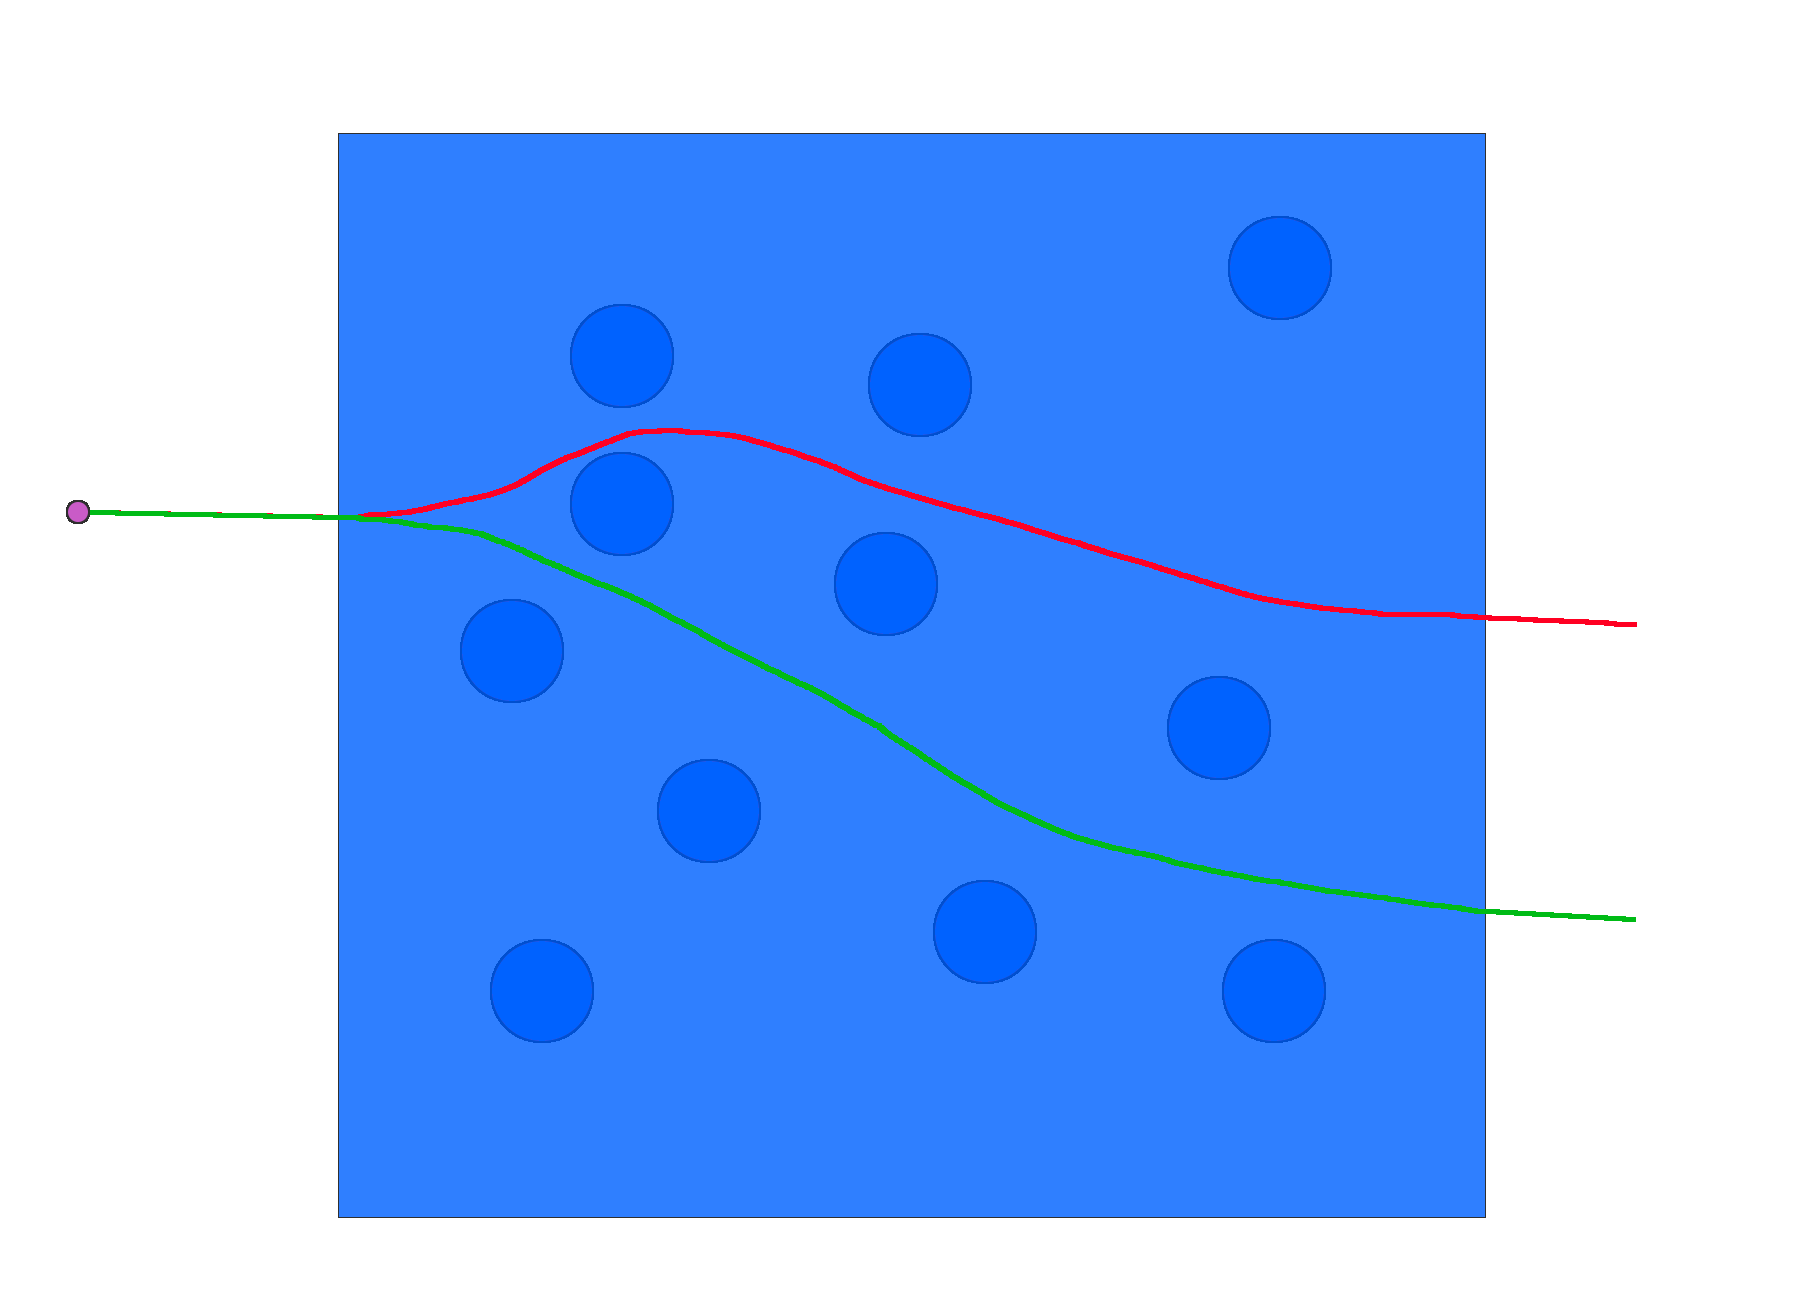
\includegraphics[width=0.75\textwidth]{Figures/lateral_displacement} 
  \caption[Two examples of true paths.]{Two examples of true paths which a particle might take when traversing a medium. Note that both the red path and green path have the same final scattered angle but different transverse positions.}
  \label{fig:lateral_displacement}
\end{figure}

For this reason, empirical corrections have been made to COSY which reflect these transverse corrections. While there is no real data on the transverse position of muons before and after they traverse a medium, it is reasonable that very small step sizes (very short true paths) should be more realistic than large step sizes. Therefore, COSY was match `empirically' with G4Beamline across several initial momenta and absorber lengths. The result was
\begin{equation}\label{eqn:cosylatdis}
x = x_o + x_D+\text{Gaus}(\theta_{diff} *L/2,\theta_c /(2\sqrt{3}),
\end{equation}
where $x_o$ is the original $x$ position, $x_D = L*P_{x,o}/P_{z,o}$ is the deterministic  gain in $x$, and Gaus($\mu,\sigma$) is a randomly selected number from a Gaussian distribution with mean $\mu$ and standard deviation $\sigma$. The forms of $\mu$ and $\sigma$ were selected based off \cite{fernowAndGallardo}. $\theta_{diff}=\theta_{final}-\theta_o$ is the amount of deflection which occurred due to scattering and $\theta_c=13.6 \text{ eV}/\beta p \cdot \sqrt{1/X_0}$ is the coefficient from Highland theory \cite{highland}.

%
%-------------------------------------------------------------------------------
%
\Section{Temporal Displacement}\label{sec:COSYTemporalDisplacement}\par
For the time-of-flight offset, both the deterministic and stochastic processes are handled in the same routine. At first order, the particle decelerates at some constant (or average) value through an absorber of length $L$. If $a$ is the constant acceleration then 
\begin{align*}
v_f=v_o+a\Delta t,
\end{align*}
or 
\begin{align*}
a=\frac{v_f-v_o}{\Delta t}.
\end{align*}
At the same time,
\begin{align*}
v_f ^2 = v_o ^2 + 2 a L,
\end{align*}
and so
\begin{align*}
a=\frac{v_f ^2 - v_o ^2}{2L}.
\end{align*}
Then
\begin{align*}
\Delta t = \frac{(v_f-v_o)2L}{v_f^2-v_o^2}.
\end{align*}
Given
\begin{align*}
\beta&=\frac{p}{E} \qquad \text{ and}\\
v&=\beta c
\end{align*}
then
\begin{equation}\label{eqn:cosyDeltaT}
\Delta t=\frac{(\frac{p_f}{E_f}-\frac{p_o}{E_o})2L}{(\frac{p_f ^2}{E_f ^2}-\frac{p_o ^2}{E_o ^2})c}.
\end{equation}

However, COSY does not have a time variable, but rather a time-like variable $\ell$, which is described as the time-of-flight in units of length. In \cite{cosy}, this is defined as
\begin{align*}
\ell=\frac{-(t-t_0)v_0\gamma}{1+\gamma},
\end{align*}
where the subscript $0$ signifies the reference particle. Let the time before a step be denoted with $1$ and the time after a step denoted with $2$. Then to find $\ell_2$ given $\ell_1$ and $\Delta t$ from Eqn. \ref{eqn:cosyDeltaT}, observe that
\begin{align} \label{eqn:cosyell12}
\begin{split}
\ell_1=\frac{(t_{01}-t_1)v_{01}\gamma_1}{1+\gamma_1} = (t_{01}-t_1)A_1\\
\ell_1=\frac{(t_{02}-t_2)v_{02}\gamma_2}{1+\gamma_2} = (t_{02}-t_2)A_2,
\end{split}
\end{align}
where 
\begin{equation}\label{eqn:cosyAn}
A_n \equiv v_{0n}\gamma_n / (1+\gamma_n).
\end{equation}
Then
\begin{align*}
\ell_2 - \ell_1 &=\big([t_{02}]-[t_2]\big)A_2-(t_{01}-t_1)A_1\\
&=\big([(t_{02}-t_{01})+t_{01}]-[(t_2-t_1)+t_1]\big)A_2-(t_{01}-t_1)A_1\\
&=(\Delta t_0 - \Delta t )A_2 + (t_{01}-t_1)A_2-(t_{01}-t_1)A_2\\
&=(\Delta t_0 - \Delta t )A_2 + (t_{01}-t_1)(A_2-A_1).
\end{align*}
Eqn. \ref{eqn:cosyell12} says that $t_{01}-t_1=\ell_1/A_1$. Moving $\ell_1$ to the right hand side,
\begin{align*}
\ell_2 &= (\Delta t_0 - \Delta t)A_2 + \frac{\ell_1}{A_1}(A_2-A_1)+\ell_1\\
&=(\Delta t_0 - \Delta t)A_2 + \ell_1\Big(\frac{A_2-A_1}{A_1}+\frac{A_1}{A_1}\Big)\\
&=(\Delta t_0 - \Delta t)A_2 + \ell_1\frac{A_2}{A_1}.
\end{align*}
Resubstituting for $A_n$ via Eqn. \ref{eqn:cosyAn} yields the final result
\begin{equation}\label{eqn:cosyell2}
\ell_2=\frac{(\Delta t_0 - \Delta t) v_{02}\gamma_2}{1+\gamma_2}+\ell_1 \frac{v_{02}\gamma_2 (1+\gamma_1)}{v_{01}\gamma_1 (1+\gamma_2)}.
\end{equation}
Using Eqn. \ref{eqn:cosyell2}, the $\Delta t$ from Eqn. \ref{eqn:cosyDeltaT} can be directly input into the new COSY variable for time-of-flight in units of length.